\documentclass[border=1cm]{standalone}
\usepackage{tikz}
\usetikzlibrary{positioning,calc}
\begin{document}
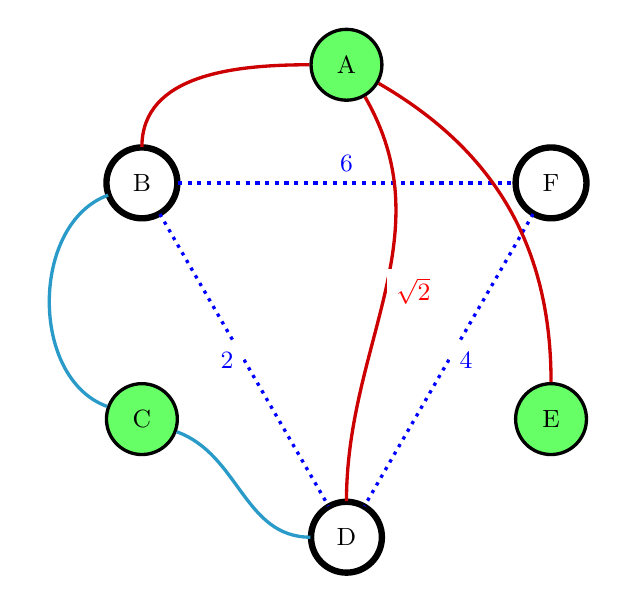
\begin{tikzpicture}[>=stealth, every node/.style={font=\small}]
  % node styles
  \tikzset{
    ring/.style={circle,draw=black,thin,double=black,double distance=1.5pt,minimum size=9mm,inner sep=0pt,fill=white},
    green/.style={circle,draw=black,very thick,minimum size=9mm,inner sep=0pt,fill=green!60},
  }

  % nodes (polar coordinates)
  \node[green] (A) at (90:3cm) {A};
  \node[ring]  (B) at (150:3cm) {B};
  \node[green] (C) at (210:3cm) {C};
  \node[ring]  (D) at (270:3cm) {D};
  \node[green] (E) at (330:3cm) {E};
  \node[ring]  (F) at (30:3cm)  {F};

  % dotted horizontal B--F with label 6 (толще)
  \draw[dotted,blue,line width=1.5pt] (B) -- node[midway,above,fill=white] {6} (F);

  % прямые линии B--D и F--D с метками 2 и 4
  \draw[dotted,blue,very thick] (B) -- node[pos=0.5,left,fill=white] {2} (D);
  \draw[dotted,blue,very thick] (F) -- node[pos=0.5,right,fill=white] {4} (D);

  % cyan curved path B--C--D
  \draw[cyan!80!black,very thick,rounded corners=6pt]
    (B) to[out=200,in=160] (C) to[out=-20,in=180] (D);

  % red smooth curve A--D with sqrt label (кривая)
  \draw[red!80!black,very thick,smooth]
    (A) to[out=-60,in=90] node[pos=0.5,right,red,fill=white] {$\sqrt{2}$} (D);
  
  % red smooth curves A--E and A--B
  \draw[red!80!black,very thick,smooth]
    (A) to[out=-30,in=90] (E);
  
  \draw[red!80!black,very thick,smooth]
    (A) to[out=180,in=90] (B);

\end{tikzpicture}
\end{document}

